%\documentclass[handout]{beamer} 
\documentclass[t,12pt,numbers,fleqn]{beamer}
%\documentclass[ignorenonframetext]{beamer}

\newif\ifquestions
%\questionstrue
\questionsfalse

\usepackage{pgfpages} 
\usepackage{hyperref}
\hypersetup{colorlinks=true,
    linkcolor=blue,
    citecolor=blue,
    filecolor=blue,
    urlcolor=blue,
    unicode=false}
\urlstyle{same}

\usepackage{booktabs}
\usepackage{multirow}

\bibliographystyle{plain}

%\usetheme{Iimenau}

\useoutertheme{split} %so the footline can be seen, without needing pgfpages

%\pgfpagesuselayout{resize to}[letterpaper,border shrink=5mm,landscape]  %if this is uncommented, the hyperref links do not work

\mode<presentation>{}

%% Requires:
%% 
%% \usepackage{latexsym}
%% \usepackage{amssymb}
%% \usepackage{stmaryrd}

%\renewcommand{\labelenumi}{(\theenumi)}

\newcommand{\be}{\begin{enumerate}}
\newcommand{\ee}{\end{enumerate}}
\newcommand{\bi}{\begin{itemize}}
\newcommand{\ei}{\end{itemize}}
\newcommand{\bc}{\begin{center}}
\newcommand{\ec}{\end{center}}
\newcommand{\bsp}{\begin{sloppypar}}
\newcommand{\esp}{\end{sloppypar}}

\newcommand{\sglsp}{\ }
\newcommand{\dblsp}{\ \ }

\newcommand{\iclicker}{i\texttt{>}clicker}

\newcommand{\sA}{\mbox{$\cal A$}}
\newcommand{\sB}{\mbox{$\cal B$}}
\newcommand{\sC}{\mbox{$\cal C$}}
\newcommand{\sD}{\mbox{$\cal D$}}
\newcommand{\sE}{\mbox{$\cal E$}}
\newcommand{\sF}{\mbox{$\cal F$}}
\newcommand{\sG}{\mbox{$\cal G$}}
\newcommand{\sH}{\mbox{$\cal H$}}
\newcommand{\sI}{\mbox{$\cal I$}}
\newcommand{\sJ}{\mbox{$\cal J$}}
\newcommand{\sK}{\mbox{$\cal K$}}
\newcommand{\sL}{\mbox{$\cal L$}}
\newcommand{\sM}{\mbox{$\cal M$}}
\newcommand{\sN}{\mbox{$\cal N$}}
\newcommand{\sO}{\mbox{$\cal O$}}
\newcommand{\sP}{\mbox{$\cal P$}}
\newcommand{\sQ}{\mbox{$\cal Q$}}
\newcommand{\sR}{\mbox{$\cal R$}}
\newcommand{\sS}{\mbox{$\cal S$}}
\newcommand{\sT}{\mbox{$\cal T$}}
\newcommand{\sU}{\mbox{$\cal U$}}
\newcommand{\sV}{\mbox{$\cal V$}}
\newcommand{\sW}{\mbox{$\cal W$}}
\newcommand{\sX}{\mbox{$\cal X$}}
\newcommand{\sY}{\mbox{$\cal Y$}}
\newcommand{\sZ}{\mbox{$\cal Z$}}

\renewcommand{\phi}{\varphi}
\newcommand{\seq}[1]{{\langle #1 \rangle}}
\newcommand{\set}[1]{{\{ #1 \}}}
\newcommand{\tuple}[1]{{( #1 )}}
\newcommand{\mlist}[1]{{[ #1 ]}}
\newcommand{\sembrack}[1]{\llbracket#1\rrbracket}
%\newcommand{\sembrack}[1]{[\![#1]\!]}
\newcommand{\synbrack}[1]{\ulcorner#1\urcorner}
\newcommand{\commabrack}[1]{\lfloor#1\rfloor}
\newcommand{\bsynbrack}[1]{\lceil#1\rceil}
\newcommand{\bsembrack}[1]{\lceil\!\!\lceil#1\rceil\!\!\rceil}
\newcommand{\mname}[1]{\mbox{\sf #1}}
\newcommand{\mcolon}{\mathrel:}
\newcommand{\mdot}{\mathrel.}
\newcommand{\modpar}{\models_{\rm par}}
\newcommand{\modreg}{\models_{\rm reg}}
\newcommand{\proves}[2]{#1 \vdash #2}
\newcommand{\notproves}[2]{#1 \not\vdash #2}
\newcommand{\provesin}[3]{#1 \vdash_{#2} #3}
\newcommand{\notprovesin}[3]{#1 \not\vdash_{#2} #3}
%\newcommand{\leqq}[1]{\mathrel{\preceq_{#1}}}
\newcommand{\parrow}{\rightharpoonup}
\newcommand{\tarrow}{\rightarrow}
\newcommand{\term}{\seq}
\newcommand{\lub}{\sqcup}
\newcommand{\subfun}{\sqsubseteq}
\newcommand{\subpred}{\subseteq}
\newcommand{\BoxApp}{\Box\,}
\newcommand{\BOX}{\mathrel{\Box}}
\newcommand{\funapp}{\mathrel@}

\newcommand{\com}{\mname{complement}}
\newcommand{\dom}{\mname{domain}}
\newcommand{\sumcl}{\mname{sum}}
\newcommand{\pow}{\mname{power}}
\newcommand{\pair}{\mname{pair}}
\newcommand{\opair}{\mname{ordered-pair}}
\newcommand{\inters}{\mname{intersection}}
\newcommand{\emp}{\mname{empty}}
\newcommand{\uni}{\mname{univocal}}
\newcommand{\fun}{\mname{function}}
\newcommand{\card}{\mname{card}}
\newcommand{\sets}{\mname{sets}}
\newcommand{\monotone}{\mname{monotone}}
\newcommand{\continuous}{\mname{continuous}}
\newcommand{\chain}{\mname{chain}}
\newcommand{\mub}{\mname{ub}}
\newcommand{\mlub}{\mname{lub}}
\newcommand{\fixedpoint}{\mname{fp}}
\newcommand{\leastfixedpoint}{\mname{lfp}}
\newcommand{\strongfixedpoint}{\mname{sfp}}
\newcommand{\emptyfun}{\triangle}
\newcommand{\statetrans}[1]{\stackrel{#1}{\longrightarrow}}
\newcommand{\thyext}{\leq}
\newcommand{\conthyext}{\unlhd}

\newcommand{\Iota}{\mbox{\rm I}}
\newcommand{\IotaApp}{\mbox{\rm I}\,}
\newcommand{\iotaApp}{\iota\,}
\newcommand{\epsilonApp}{\epsilon\,}
\newcommand{\True}{\mbox{\sf T}} 
\newcommand{\False}{\mbox{\sf F}} 
\newcommand{\Trueword}{\sf true}
\newcommand{\Falseword}{\sf false}
\newcommand{\Neg}{\neg} 
\newcommand{\Andd}{\wedge}
\newcommand{\Or}{\vee}
\newcommand{\Implies}{\supset}
\newcommand{\ImpliesAlt}{\Rightarrow}
\newcommand{\Iff}{\equiv}
\newcommand{\Sheffer}{\mathrel|}
\newcommand{\IffAlt}{\Leftrightarrow}
\newcommand{\Forall}{\forall}
\newcommand{\ForallApp}{\forall\,}
\newcommand{\Forsome}{\exists}
\newcommand{\ForsomeApp}{\exists\,}
\newcommand{\ForsomeUniqueApp}{\exists\,!\,}
\newcommand{\IsDef}{\downarrow}
\newcommand{\IsUndef}{\uparrow}
\newcommand{\Equal}{=}
\newcommand{\QuasiEqual}{\simeq}
\newcommand{\Undefined}{\bot}
\newcommand{\If}{\mname{if}}
\newcommand{\IsDefApp}{\!\IsDef}
\newcommand{\IsUndefApp}{\!\IsUndef}
\newcommand{\TRUE}{\mbox{{\sc t}}}
\newcommand{\FALSE}{\mbox{{\sc f}}}
\newcommand{\truthvalues}{\{\TRUE,\FALSE\}}
\newcommand{\LambdaApp}{\lambda\,}
\newcommand{\LAMBDAapp}{\Lambda\,}
\newcommand{\AlphaEquiv}{\stackrel{\alpha}{=}}

\newcommand{\mvar}[3]{\textbf{var}_{#1}[#2,#3]}
\newcommand{\mterm}[2]{\textbf{term}_{#1}[#2]}
\newcommand{\mform}[2]{\textbf{form}_{#1}[#2]}
\newcommand{\mtype}[2]{\textbf{type}_{#1}[#2]}
\newcommand{\mexpr}[3]{\textbf{expr}_{#1}[#2,#3]}

\newcommand{\imps}{\mbox{\sc imps}}
\newcommand{\fol}{\mbox{\sc fol}}
\newcommand{\lutins}{\mbox{\sc lutins}}
\newcommand{\vlisp}{\mbox{\sc vlisp}}
\newcommand{\vmach}{\mbox{\sc vmach}}
\newcommand{\gnu}{\mbox{\sc gnu}}
\newcommand{\zf}{\mbox{\sc zf}}
\newcommand{\nbg}{\mbox{\sc nbg}}
\newcommand{\pnbg}{\mbox{\sc pnbg}}
\newcommand{\snbg}{\mbox{\sc snbg}}
\newcommand{\pfol}{\mbox{\sc pfol}}
\newcommand{\nbgstar}{$\mbox{\sc nbg}^\ast$}
\newcommand{\boldnbgstar}{$\mbox{\bf NBG}^\ast$}
\newcommand{\stt}{\mbox{\sc stt}}
\newcommand{\eves}{\mbox{\sc eves}}
\newcommand{\hol}{\mbox{\sc hol}}
\newcommand{\mizar}{Mizar}
\newcommand{\nqthm}{Nqthm}
\newcommand{\pvs}{\mbox{\sc pvs}}
\newcommand{\stmm}{\mbox{\sc stmm}}

\iffalse
\newtheorem{thm}{Theorem}[section]
\newtheorem{cor}[thm]{Corollary}
\newtheorem{lem}[thm]{Lemma}
\newtheorem{prop}[thm]{Proposition}
\newtheorem{rem}[thm]{Remark}
\newtheorem{eg}[thm]{Example}
\newtheorem{df}[thm]{Definition}
\fi

%\newenvironment{proof}{\par\noindent{\bf Proof\ \ }}{$\Box$}

\newenvironment{namedform}[1]
   {\begin{tabbing}\textbf{#1}\ }
   {\end{tabbing}}

\newcommand{\urlpart}[1]{\mbox{\texttt{#1}}\linebreak[0]}

\newcommand{\bblue}{\textcolor{blue!80!black}}
\newcommand{\bgreen}{\textcolor{green!55!black}}
\newcommand{\bbrown}{\textcolor{brown}}
\newcommand{\bred}{\textcolor{red!80!black}}
\newcommand{\bcyan}{\textcolor{cyan!80!black}}
\newcommand{\bmagenta}{\textcolor{magenta}}
\newcommand{\byellow}{\textcolor{yellow}}
\newcommand{\borange}{\textcolor{orange}}
\newcommand{\bviolet}{\textcolor{violet}}
\newcommand{\bpurple}{\textcolor{purple}}
\newcommand{\bdarkgray}{\textcolor{darkgray}}
\newcommand{\bgray}{\textcolor{gray}}
\newcommand{\blightgray}{\textcolor{lightgray}}

\newcommand{\clicker}{i\texttt{>}clicker}

\newenvironment{changemargin}[2]{%
  \begin{list}{}{%
    \setlength{\topsep}{0pt}%
    \setlength{\leftmargin}{#1}%
    \setlength{\rightmargin}{#2}%
    \setlength{\listparindent}{\parindent}%
    \setlength{\itemindent}{\parindent}%
    \setlength{\parsep}{\parskip}%
  }%
  \item[]}{\end{list}}


\newcommand{\topic}{13 Modular Design}

%Title page information for 1D04 lectures slides

% Define year specific parameters - used in title page and footer

\newcommand{\season}{Fall} %use to switch between Winter and Fall
\newcommand{\instructor}{Dr.~Spencer Smith} %use to switch instructor
\newcommand{\instructSmall}{Dr.~Smith}
\newcommand{\yr}{2019}
\newcommand{\courseCode}{CAS 741, CES 741}
\newcommand{\courseTitle}{Development of Scientific Computing Software}

%\setbeamerfont{structure}{series=\bfseries}
%\usefonttheme[stillsansseriftext,stillsansserifmath]{serif}
\setbeamertemplate{navigation symbols}{} 
\setbeamertemplate{itemize item}[ball]

\title{
  {\normalsize \bf 
    \borange{\courseCode~(\courseTitle)\\ \season~\yr}}\\[2ex]
  {\Large \bf \topic}}

\author[Smith]{\instructor}

\institute{
  Faculty of Engineering,
  McMaster University}

\date{
\today
%January 2011\\
\bc
  
\includegraphics[scale = 0.2, keepaspectratio]
  {../mcmaster-logo-full-color.jpg}
\ec
}

\renewcommand{\borange}[1] %orange is too hard to read
{
   \bred{#1}
}

\begin{document}

% Footline for  Slides

% Display title page and displays footers

\setbeamertemplate{footline}{} %so the title screen does not have a footline

%%%%%%%%%%%%%%%%%%%%%%%%%%%%%%%%%%%%%%%%%%%%%%%%%%%%%%%%%%%%

\begin{frame}
\titlepage
\end{frame}

%%%%%%%%%%%%%%%%%%%%%%%%%%%%%%%%%%%%%%%%%%%%%%%%%%%%%%

\setbeamertemplate{footline}{
\begin{beamercolorbox}{sectioninhead/foot}
\hspace{1ex}\bblue{\hrulefill}\hspace{1ex}

\vspace{1ex}
\hspace{1ex}
{\tiny \instructSmall \hfill 
\courseCode~\season~\yr:~\topic \hfill 
\insertframenumber/\inserttotalframenumber~~}
%\insertframenumber/\ref{lastframe}}
%\hfill {\small \insertframenumber} \hspace{10ex}
%{\small $$\insertframenumber$$}
\vspace{1ex}
\end{beamercolorbox}}

%%%%%%%%%%%%%%%%%%%%%%%%%%%%%%%%%%%%%%%%%%%%%%%%%%%%%%


%%%%%%%%%%%%%%%%%%%%%%%%%%%%%%%%%%%%%%%%%%%%%%%%%%%%%%

\begin{frame}
\frametitle{Modular Design}

\bi
\item Administrative details
\item Questions?
%\item Feedback on SRS
\item Overview of design
\item Modular decomposition: advantages, guidelines etc.
\item Module guide
\item Module guide example
\item Integration Testing 
\ei
\end{frame}

%%%%%%%%%%%%%%%%%%%%%%%%%%%%%%%%%%%%%%%%%%%%%%%%%%%%%%

\begin{frame}
\frametitle{Administrative Details}

\bi
%\item GitHub issues
%\bi
% \item When closing issues give the hash for the corresponding commit
% \item Everyone should have an issue to review my comments on their SRS or CA
% \ei
\item VnV GitHub issues for colleagues
\bi
\item Assigned 1 colleague (see \texttt{Repos.xlsx} in repo)
\item Provide at least 5 issues on their VnV Plan
\item Grading as before
\item Due by Friday, Oct 26, 11:59 pm
\item If you have an extension past today, please let your partner know
\item If your partner has an extension, you have three days after their deadline
\ei

%\item For MG presentation, we'll try to use my laptop only
\item Grading scheme for VnV now available on Avenue
\item Template for MG updated in repo
\ei

\end{frame}

%%%%%%%%%%%%%%%%%%%%%%%%%%%%%%%%%%%%%%%%%%%%%%%%%%%%%%

\begin{frame}
\frametitle{Administrative Details: Deadlines}

~\newline
\begin{tabular}{l l l}
\textbf{MG Present} & Week 08 & Week of Oct 29\\
\textbf{MG} & Week 09 & Nov 5\\
MIS Present & Week 10 & Week of Nov 12\\
MIS & Week 11 & Nov 19\\
Unit VnV or Impl.\ Present & Week 12 & Week of Nov 26\\
Unit VnV Plan & Week 13 & Dec 3\\
Final Doc & Week 14 & Dec 10\\
\end {tabular}

\end{frame}

%%%%%%%%%%%%%%%%%%%%%%%%%%%%%%%%%%%%%%%%%%%%%%%%%%%%%%

\begin{frame}
\frametitle{Administrative Details: Presentation Schedule}

\bi
\item MG Present
\bi
\item \textbf{Wednesday: Karol, Malavika, Robert, Hanane}
\item \textbf{Friday: Brooks, Vajiheh, Olu, Jennifer}
\ei
\item MIS Present
\bi
\item Wednesday: Malavika, Robert
\item Friday: Hanane,  Jennifer
\ei
\item Unit VnV Plan or Impl.\ Present
\bi
\item Wednesday: Brooks, Vajiheh
\item Friday: Olu, Karol
\ei
\ei

\end{frame}

%%%%%%%%%%%%%%%%%%%%%%%%%%%%%%%%%%%%%%%%%%%%%%%%%%%%%%

\begin{frame}
\frametitle{Questions?}
\begin{itemize}
\item \structure{Questions about Verification and Validation plan?}
\end{itemize}
\end{frame}

%%%%%%%%%%%%%%%%%%%%%%%%%%%%%%%%%%%%%%%%%%%%%%%%%%%%%%

% \begin{frame}
% \frametitle{Feedback on SRS}
% \begin{itemize}
% \item Overall well done!
% \item Don't need padding (\textbf{Watch for MG!})
% \bi
% \item Don't make more complicated than it is
% \item Don't add assumptions that the data will be in the correct format, or of
%   the correct type 
% \ei
% \item For the characteristics of intended reader try to be more specific about
%   the education.  What degree?  What course areas?  What level?
% \item If you have a reference by entry, then the referenced by chunk (or its
%   derivation) should actually reference the chunk that has it as an entry.
% \item Functional requirements should reference the instance models
% \item Add more for nonfunctional requirements
% \item Introduce type information when it will help clarify spec
% \end{itemize}
% \end{frame}

% %%%%%%%%%%%%%%%%%%%%%%%%%%%%%%%%%%%%%%%%%%%%%%%%%%%%%

% \begin{frame}[fragile]
% \frametitle{LaTeX Related Feedback}
% \bi
% \item The text is better for version control, and for reading in other editors,
%   if you use a hard-wrap at 80 characters
% \item Use \verb|``quote''| to get correct quotation marks
% \item Spell check!
% \item Check for extra and missing spaces
% \item LaTeX often inserts two spaces after a period, use \verb|Dr.\ Jeckyl| or
%   \verb|Dr.~Jeckyl|
% \item For $ABC_{Average}$ in an equation use
%   \verb|$\mathit{ABC}_{\text{Average}}$| ($\mathit{ABC}_{\text{Average}}$)
% \item Use BibTeX.  You should mention the source of the
%   template~\cite{SmithAndLai2005, SmithEtAl2007} 
% \item Cite all sources!
% \ei
% \end{frame}

%%%%%%%%%%%%%%%%%%%%%%%%%%%%%%%%%%%%%%%%%%%%%%%%%%%%%%

\begin{frame}

\frametitle{Review of our ``Faked'' Rational Design Process}

\begin{center}
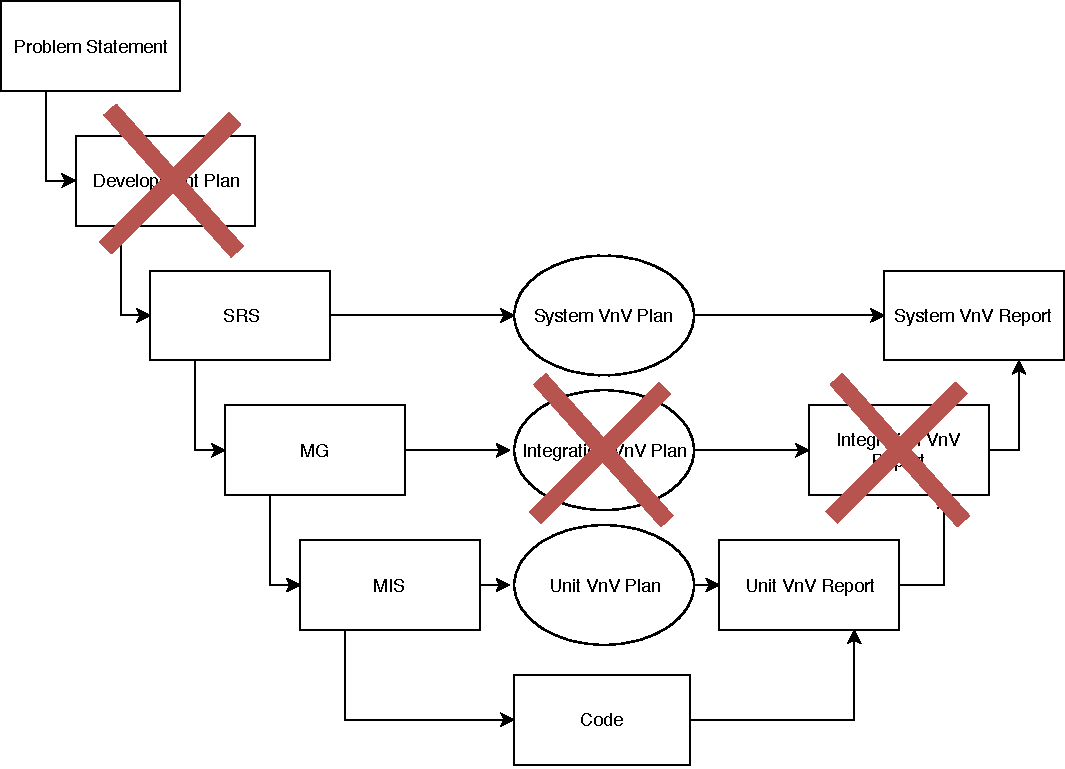
\includegraphics[scale=0.55]{../Figures/VModelOfProcessXOut.pdf}
\end{center}

\end{frame}

%%%%%%%%%%%%%%%%%%%%%%%%%%%%%%%%%%%%%%%%%%%%%%%%%%%%%%

\begin{frame}
\frametitle{SWHS MG Example}
~\\
\href{https://github.com/smiths/swhs/tree/master/docs/Design/MG}
{https://github.com/smiths/swhs/tree/master/docs/Design/MG}
\end{frame}

%%%%%%%%%%%%%%%%%%%%%%%%%%%%%%%%%%%%%%%%%%%%%%%%%%%%%%

\begin{frame}
\frametitle{What is Design?}
\begin{itemize}
\item Your requirements document identifies ``What,'' now we begin to look at ``How''
\item Your system should meet both your functional and nonfunctional requirements
\item There is no unique ``optimal'' design
\begin{itemize}
\item Different goals will lead to different designs
\item There is a mix of art and science in design
\item Even with fully formal requirements specification there does not yet exist a systematic way to obtain a design
\item Favour art in some areas and favour science in others
\end{itemize}
\end{itemize}
\end{frame}

%%%%%%%%%%%%%%%%%%%%%%%%%%%%%%%%%%%%%%%%%%%%%%%%%%%%%%

\begin{frame}
\frametitle{What is Design Continued?}

\begin{itemize}

\item Provides structure to any artifact
\item Decomposes system into parts, assigns responsibilities, ensures that parts
  fit together to achieve a global goal
\item Design refers to
\bi
\item Activity
\bi
\item Bridge between requirements and implementation
\item Structure to an artifact
\ei
\item Result of the activity
\bi
\item System decomposition into modules (module guide)
\item Module interface specification (MIS)
\ei
\end{itemize}
\end{itemize}

\end{frame}

%%%%%%%%%%%%%%%%%%%%%%%%%%%%%%%%%%%%%%%%%%%%%%%%%%%%%%

\begin{frame}
\frametitle{Why Decompose Into Modules?}

\begin{itemize}
\item Separation of concerns
\item Cannot understand all of the details
\item All engineering fields use decomposition
\item Modules will act as ``work assignments''
\item Decomposition needs to follow a systematic procedure (as for SRS)
\item Need to ensure that modules when fit together achieve our global goals
\item Document in a Software Design Document (Module Guide)
\end{itemize}

\end{frame}

%%%%%%%%%%%%%%%%%%%%%%%%%%%%%%%%%%%%%%%%%%%%%%%%%%%%%%

\begin{frame}
\frametitle{Benefits of Modularity}
\begin{itemize}
\item Shorter development time
\item Improved verification
\item Reduced maintenance costs
\item Easier to understand
\begin{itemize}
\item Small modules
\item An abstract interface
\end{itemize}
\item Modules can be developed independently
\item Modules can be tested independently
\item Modules can be reused
\item Software is easy to change, extend, maintain
\item This requires identifying the anticipated changes in the design and in the requirements
\end{itemize}
\end{frame}

%%%%%%%%%%%%%%%%%%%%%%%%%%%%%%%%%%%%%%%%%%%%%%%%%%%%%%

\begin{frame}
\frametitle{Two Important Goals for Decomposition}

\begin{itemize}

\item Design for change (Parnas) \cite{Parnas1972a, Parnas1974}
\bi
\item Designers tend to concentrate on current needs
\item Special effort needed to anticipate likely changes
\item Changes can be in the design or in the requirements
\item Too expensive to design for all changes, but should design for likely
  changes
\ei
\item Product families (Parnas) \cite{Parnas1976, Parnas1979}
\bi
\item Think of the current system under design as a member of a program family
\item Analogous to product lines in other engineering disciplines
\item Example product families include automobiles, cell phones, etc.
\item Design the whole family as one system, not each individual family member
  separately 
\ei
\end{itemize}

Use Design Principle of Information Hiding

\end{frame}

%%%%%%%%%%%%%%%%%%%%%%%%%%%%%%%%%%%%%%%%%%%%%%%%%%%%%%

\begin{frame}
\frametitle{Sample Likely Changes}

What are some examples of likely changes for software?

\end{frame}

%%%%%%%%%%%%%%%%%%%%%%%%%%%%%%%%%%%%%%%%%%%%%%%%%%%%%%7

\begin{frame}
\frametitle{Sample Likely Changes \cite{GhezziEtAl2003}}

\begin{itemize}

\item Algorithms -- like replacing inefficient sorting algorithm with a more
  efficient one
\item Change of data representation
\bi
\item From binary tree to threaded tree
\item Array implementation to a pointer implementation
\item Approx.\ 17\% of maintenance costs attributed to data representation
  changes (Lientz and Swanson, 1980)
\ei
\item Change of underlying abstract machine
\bi
\item New release of operating system
\item New optimizing compiler
\item New version of DBMS
\item etc.
\ei
\item Change of peripheral devices

\end{itemize}

\end{frame}

%%%%%%%%%%%%%%%%%%%%%%%%%%%%%%%%%%%%%%%%%%%%%%%%%%%%%%

\begin{frame}
\frametitle{Binary Tree to Threaded Tree}

%\vspace{-2cm}
\begin{center}
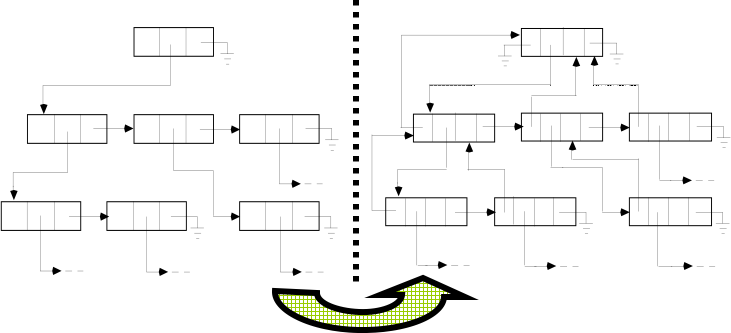
\includegraphics[width=1.1\textwidth]{../Figures/BinTreeToThreadTree.png}
\end{center}

\end{frame}

%%%%%%%%%%%%%%%%%%%%%%%%%%%%%%%%%%%%%%%%%%%%%%%%%%%%%%

\begin{frame}
\frametitle{Sample Likely Changes}

\begin{itemize}

\item Change of ``social'' environment
\bi
\item Corresponds to requirements changes
\item New tax regime
\item EURO versus national currency in EU
\item New language for user interface
\item y2k
\ei
\item Change due to development process (prototype transformed into product)

\end{itemize}

\end{frame}

%%%%%%%%%%%%%%%%%%%%%%%%%%%%%%%%%%%%%%%%%%%%%%%%%%%%%%

\begin{frame}
\frametitle{Components of a Module}

\begin{itemize}

\item A software modules has two components
\begin{enumerate}
\item An \structure{interface} that enables the module's clients to use the
  service the module provides
\item An \structure{implementation} of the interface that provides the services
  offered by the module
\end{enumerate}

\end{itemize}

\end{frame}

%%%%%%%%%%%%%%%%%%%%%%%%%%%%%%%%%%%%%%%%%%%%%%%%%%%%%%

\begin{frame}
\frametitle{The Module Interface}

\begin{itemize}

\item A module's interface can be viewed in various ways
\begin{itemize}
\item As a \structure{set of services}
\item As a \structure{contract} between the module and its clients
\item As a \structure{language} for using the module's services
\end{itemize}
\item The interface is \structure{exported} by the module and
  \structure{imported} by the module's clients
\item An interface describes the \structure{data} and \structure{procedures}
  that provide access to the services of the module

\end{itemize}

\end{frame}

%%%%%%%%%%%%%%%%%%%%%%%%%%%%%%%%%%%%%%%%%%%%%%%%%%%%%%

\begin{frame}
\frametitle{The Module Implementation}

\begin{itemize}

\item A module's implementation is an implementation of the module's interface
\item The implementation is \structure{hidden} from other modules
\item The interface data and procedures are implemented together and may share
  data structures
\item The implementation may utilize the services offered by other modules

\end{itemize}

\end{frame}

%%%%%%%%%%%%%%%%%%%%%%%%%%%%%%%%%%%%%%%%%%%%%%%%%%%%%%

\begin{frame}
\frametitle{Information Hiding}

\begin{itemize}

\item Made explicit by Parnas \cite{Parnas1972a}
\item Basis for design (that is modular decomposition (Module Guide))
\item Implementation secrets are hidden to clients
\item Secret can be changed freely if the change does not affect the interface
\item \structure{Try to encapsulate changeable design decisions as
    implementation secrets within module implementations}

\end{itemize}

\end{frame}

%%%%%%%%%%%%%%%%%%%%%%%%%%%%%%%%%%%%%%%%%%%%%%%%%%%%%%

\begin{frame}
\frametitle{Examples of Modules \cite{GhezziEtAl2003}}

\begin{itemize}

\item \structure{Record}
\begin{itemize}
\item Consists of only data
\item Has state but no behaviour
\end{itemize}
\item \structure{Collection of related procedures (library)}
\begin{itemize}
\item Has behaviour but no state
\item Procedural abstractions
% like many routines in a scientific computing library
\end{itemize}
\item \structure{Abstract object}
\begin{itemize}
\item Consists of data (\structure{fields}) and procedures (\structure{methods})
\item Consists of a collection of \structure{constructors},
  \structure{selectors}, and \structure{mutators}
\item Has state and behaviour
\end{itemize}
\end{itemize}

\end{frame}

%%%%%%%%%%%%%%%%%%%%%%%%%%%%%%%%%%%%%%%%%%%%%%%%%%%%%%

\begin{frame}
\frametitle{Examples of Modules Continued}

\begin{itemize}

\item \structure{Abstract data type (ADT)}
\begin{itemize}
\item Consists of a collection of abstract objects and a collection of
  procedures that can be applied to them
\item Defines the set of possible values for the type and the associated
  procedures that manipulate instances of the type
\item Encapsulates the details of the implementation of the type
\end{itemize}
\item \structure{Generic Modules}
\begin{itemize}
\item A single abstract description for a family of abstract objects or ADTs
\item Parameterized by type
\item Eliminates the need for writing similar specifications for modules that
  only differ in their type information
\item A generic module facilitates specification of a stack of integers, stack
  of strings, stack of stacks etc.
\end{itemize}

\end{itemize}

\end{frame}

%%%%%%%%%%%%%%%%%%%%%%%%%%%%%%%%%%%%%%%%%%%%%%%%%%%%%%

% \begin{frame}
% \frametitle{Specific Techniques for Design for Change}

% What software tool would you use if you wanted to select at build time between
% two implementations of a module, each distinguished by a different decision for
% their shared secret?

% \end{frame}

% %%%%%%%%%%%%%%%%%%%%%%%%%%%%%%%%%%%%%%%%%%%%%%%%%%%%%%

% \begin{frame}
% \frametitle{Specific Techniques for Design for Change}

% \begin{itemize}
% \item Anticipate definition of all family members
% \item Identify what is common to all family members, delay decisions that
%   differentiate among different members
% \item Configuration constants
% \begin{itemize}
% \item Factor constant values into symbolic constants
% \item Compile time binding
% \item MAXSPEED = 5600
% \end{itemize}
% \item Conditional compilation
% \bi
% \item Compile time binding
% \item Works well when there is a preprocessor, like for C
% \item If performance is not a concern, can often ``fake it'' at run time
% \ei
% \item Make
% \item Software generation
% \bi
% \item Compiler generator, like \texttt{yacc}
% \item Domain Specific Language
% \ei
% \end{itemize}

% \end{frame}

%%%%%%%%%%%%%%%%%%%%%%%%%%%%%%%%%%%%%%%%%%%%%%%%%%%%%%

\begin{frame}
\frametitle{Questions}

\begin{itemize}
\item What relationships are there between modules?
\item Are there desirable properties for these relations?
\end{itemize}

\end{frame}

%%%%%%%%%%%%%%%%%%%%%%%%%%%%%%%%%%%%%%%%%%%%%%%%%%%%%%

\begin{frame}
\frametitle{Relationships Between Modules \cite{GhezziEtAl2003}}

\begin{itemize}
\item Let $S$ be a set of modules
$$ S = \{ M_1, M_2, ..., M_n \}$$
\item A binary relation $r$ on $S$ is a subset of $S \times S$
\item If $M_i$ and $M_j$ are in $S$, $< M_i, M_j > \in r$ can be written as $M_i r M_j$
\end{itemize} 

\end{frame}

%%%%%%%%%%%%%%%%%%%%%%%%%%%%%%%%%%%%%%%%%%%%%%%%%%%%%%

\begin{frame}
\frametitle{Relations}

\begin{itemize}
\item Transitive closure $r^{+}$ of $r$
$$M_i r^{+} M_j \mbox{ iff } M_i r M_j \mbox{ or } \exists M_k \mbox{ in } S \mbox{ such that } M_i r M_k \mbox{ and } M_k
r^{+} M_j$$
\item $r$ is a hierarchy iff there are no two elements $M_i$, $M_j$ such that
  $M_i r^{+} M_j \wedge M_j r^{+} M_i$
\end{itemize}

\end{frame}

%%%%%%%%%%%%%%%%%%%%%%%%%%%%%%%%%%%%%%%%%%%%%%%%%%%%%%

\begin{frame}
\frametitle{Relations Continued}

\begin{itemize}
\item Relations can be represented as graphs
\item A hierarchy is a DAG (Directed Acyclic Graph)
\end{itemize}

\begin{center}
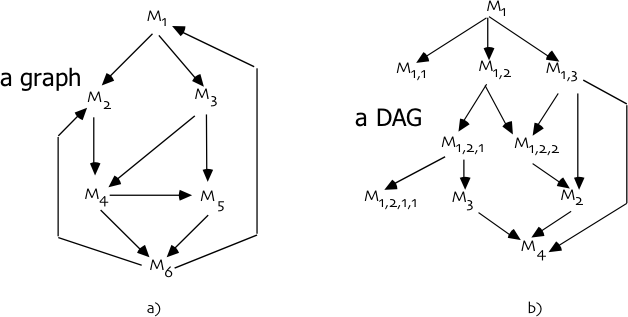
\includegraphics[width=1.0\textwidth]{../Figures/GraphAndDAG.png}
\end{center}

\structure{Why do we prefer the uses relation to be a DAG?}

\end{frame}

%%%%%%%%%%%%%%%%%%%%%%%%%%%%%%%%%%%%%%%%%%%%%%%%%%%%%%

\begin{frame}
\frametitle{Desirable Properties}

\begin{itemize}
\item USES should be a hierarchy \cite{Parnas1974}
\begin{itemize}
\item Hierarchy makes software easier to understand
\item We can proceed from the leaf nodes (nodes that do not use other nodes)
  upwards
\item They make software easier to build
\item They make software easier to test
\end{itemize}
\item Low coupling
\item Fan-in is considered better than Fan-out: \structure{WHY?}
\end{itemize}

\end{frame}

%%%%%%%%%%%%%%%%%%%%%%%%%%%%%%%%%%%%%%%%%%%%%%%%%%%%%%

\begin{frame}
\frametitle{DAG Versus Tree}

Is a DAG a tree?  Is a tree a DAG?

\end{frame}

%%%%%%%%%%%%%%%%%%%%%%%%%%%%%%%%%%%%%%%%%%%%%%%%%%%%%%

\begin{frame}
\frametitle{DAG Versus Tree}

Would you prefer your uses relation is a tree?

\end{frame}

%%%%%%%%%%%%%%%%%%%%%%%%%%%%%%%%%%%%%%%%%%%%%%%%%%%%%%

\begin{frame}
\frametitle{Hierarchy}

\begin{itemize}
\item Organizes the modular structure through \structure{levels of abstraction}
\item Each level defines an \structure{abstract (virtual) machine} for the next level
\item Level can be defined precisely
\begin{itemize}
\item $M_i$ has level $0$ if no $M_j$ exists such that $M_i r M_j$
\item Let $k$ be the maximum level of all nodes $M_j$ such that $M_i r M_j$, then $M_i$ has level $k+1$
\end{itemize}
\end{itemize}

\end{frame}

%%%%%%%%%%%%%%%%%%%%%%%%%%%%%%%%%%%%%%%%%%%%%%%%%%%%%%%%%%%%%%%%%%%%%%%%%%%%%

\begin{frame}
\frametitle{Static Definition of Uses Relation}

Your program has code like:\\
\texttt{if cond then ServiceFromMod1 else ServiceFromMod2}\\
~\newline
This is the only place where each module is used.  Does this mean the uses
relation depends on the dynamic execution of the program?
\end{frame}

%%%%%%%%%%%%%%%%%%%%%%%%%%%%%%%%%%%%%%%%%%%%%%%%%%%%%%

\begin{frame}
\frametitle{Question about Association and DAG}

\structure{Is the uses relation here a DAG?}\\

\begin{figure}
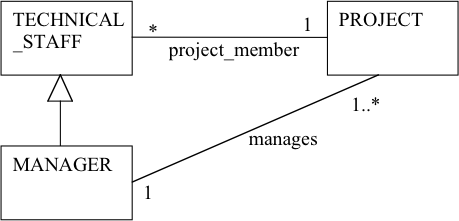
\includegraphics[scale=0.6]{../Figures/UML_Association.png}
\end{figure}

\end{frame}

%%%%%%%%%%%%%%%%%%%%%%%%%%%%%%%%%%%%%%%%%%%%%%%%%%%%%%

\begin{frame}
\frametitle{Module Decomposition (Parnas)}

\begin{center}
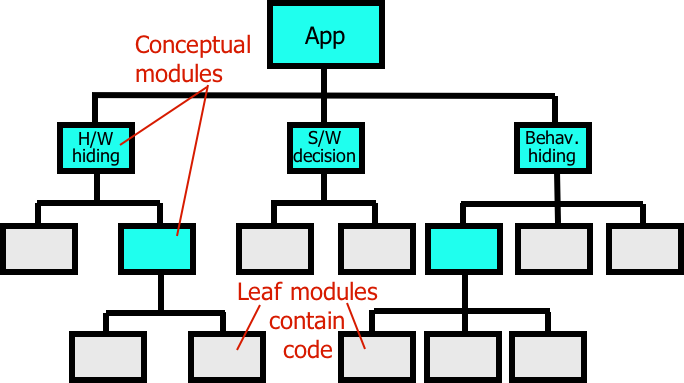
\includegraphics[width=1.0\textwidth]{../Figures/ParnasDecompBySecrets.png}
\end{center}

\end{frame}

%%%%%%%%%%%%%%%%%%%%%%%%%%%%%%%%%%%%%%%%%%%%%%%%%%%%%%

\begin{frame}
\frametitle{Module Decomposition (Parnas)}

For the module decomposition on the previous slide:

\begin{itemize}
\item Does it show a Uses relation?  
\item Is it a DAG?  
\item Is it a tree?
\end{itemize}

\end{frame}

%%%%%%%%%%%%%%%%%%%%%%%%%%%%%%%%%%%%%%%%%%%%%%%%%%%%%%

\begin{frame}
\frametitle{IS\_COMPONENT\_OF}

\begin{itemize}
\item The Parnas decomposition by secrets gives an IS\_COMPONENT\_OF relationship
\item Used to describe a higher level module as constituted by a number of lower level modules
\item A IS\_COMPONENT\_OF B means B consists of several modules of which one is A
\item B COMPRISES A
\item $M_{S,i} = \{ M_k | M_k \in S \wedge M_k \mbox{ IS\_COMPONENT\_OF } M_i \}$ we say that $M_{S,i}$ IMPLEMENTS
$M_i$ 
%\item \structure{How is IS\_COMPONENT\_OF represented in UML?}
\end{itemize}

\end{frame}

%%%%%%%%%%%%%%%%%%%%%%%%%%%%%%%%%%%%%%%%%%%%%%%%%%%%%%

\begin{frame}
\frametitle{A Graphical View}

\begin{center}
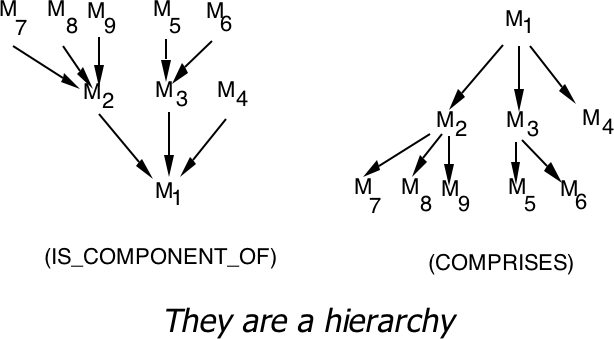
\includegraphics[width=1.0\textwidth]{../Figures/GraphViewOf_IS_COMPONENT_OF.png}
\end{center}

\end{frame}

%%%%%%%%%%%%%%%%%%%%%%%%%%%%%%%%%%%%%%%%%%%%%%%%%%%%%%

% \begin{frame}
% \frametitle{Product Families}

% \begin{itemize}
% \item Careful recording of (hierarchical) USES relation and IS\_COMPONENT\_OF supports design of program families
% \item Attempt to recognize modules that will differ in implementation between family members
% \item New program family member should start at the documentation of the design, not with the code
% \end{itemize}

% \end{frame}

%%%%%%%%%%%%%%%%%%%%%%%%%%%%%%%%%%%%%%%%%%%%%%%%%%%%%%

% \begin{frame}
% \frametitle{Remember - Information Hiding}

% \begin{itemize}
% \item Basis for design (i.e.\ module decomposition)
% \item Implementation secrets are hidden to clients
% \item They can be changed freely if the change does not affect the interface
% \item \structure{Try to encapsulate changeable requirements and design decisions as implementation secrets within module
% implementations}
% \item Decomposition by secrets, not by sequence of steps
% \end{itemize}

% \end{frame}

% %%%%%%%%%%%%%%%%%%%%%%%%%%%%%%%%%%%%%%%%%%%%%%%%%%%%%%

% \begin{frame}
% \frametitle{Prototyping}

% \begin{itemize}
% \item Once an interface is defined, implementation can be done
% \begin{itemize}
% \item First quickly but inefficiently
% \item Then progressively turned into the final version
% \end{itemize}
% \item Initial version acts as a prototype that evolves into the final product
% \end{itemize}

% \end{frame}

%%%%%%%%%%%%%%%%%%%%%%%%%%%%%%%%%%%%%%%%%%%%%%%%%%%%%%

% \begin{frame}
% \frametitle{Parnas's Rational Design Process (RDP)}

% \begin{itemize}
% \item SRS
% \item MG
% \item Uses Hierarchy (updated after writing MISes)
% \item For each module
% \begin{itemize} 
% \item MIS
% \item MID (we will not emphasize this document)
% \end{itemize}
% \item Implementation
% \item Testing
% \item Very successfully used on projects such as 
% \begin{itemize}
% \item The Darlington Nuclear Reactor shutdown system
% \item The A7-E fighter jet
% \end{itemize}
% \end{itemize}

% \end{frame}

%%%%%%%%%%%%%%%%%%%%%%%%%%%%%%%%%%%%%%%%%%%%%%%%%%%%%%

\begin{frame}
\frametitle{Module Guide \cite{ParnasEtAl1984}}

\begin{itemize}
\item Part of Parnas' Rational Design Process (RDP)
\item When decomposing the system into modules, we need to document the module
  decomposition so that developers and other readers can understand and verify
  the decomposition
\item Helps future maintainers find appropriate module
\item Parnas proposed a Module Guide (MG) based on the decomposition module tree
  shown earlier
\item Decomposition is usually three to five levels deep
\end{itemize}

\end{frame}

%%%%%%%%%%%%%%%%%%%%%%%%%%%%%%%%%%%%%%%%%%%%%%%%%%%%%%

\begin{frame}
\frametitle{Three Top Conceptual Modules in an RDP MG}

\structure{What are the three groups of modules in a typical information-hiding
  decomposition?}

\end{frame}

%%%%%%%%%%%%%%%%%%%%%%%%%%%%%%%%%%%%%%%%%%%%%%%%%%%%%%

\begin{frame}
\frametitle{Module Decomposition (Parnas)}

\begin{center}
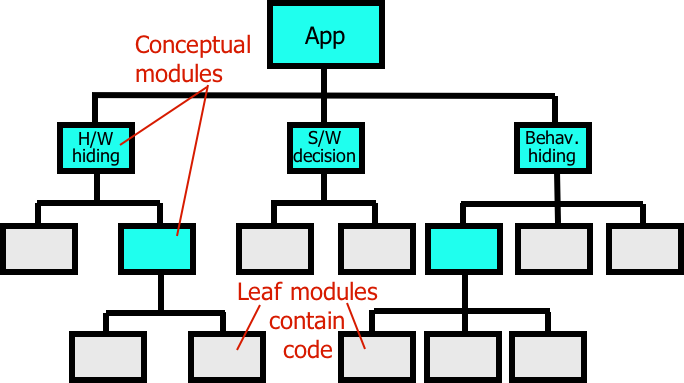
\includegraphics[width=1.0\textwidth]{../Figures/ParnasDecompBySecrets.png}
\end{center}

\end{frame}

%%%%%%%%%%%%%%%%%%%%%%%%%%%%%%%%%%%%%%%%%%%%%%%%%%%%%%

\begin{frame}
\frametitle{RDP - MG}

\begin{itemize}
\item The MG consists of a table that documents each module's service and secret
\item Conceptual modules will have broader responsibilities and secrets
\item Following a particular branch, the secrets at lower levels ``sum up'' to
  the secret at higher levels
\item The leaf modules that represent code will contain much more precise
  services and secrets
\item Only the leaf modules are actually implemented
\item The MG should list the likely and unlikely changes on which the design is based
\end{itemize}

\end{frame}

%%%%%%%%%%%%%%%%%%%%%%%%%%%%%%%%%%%%%%%%%%%%%%%%%%%%%%

\begin{frame}
\frametitle{Module Details}
\begin{itemize}
\item For each module
\item Module name
\item Secret (informal description)
\item Service or responsibility (informal description)
\item For ``leaf'' modules add
\begin{itemize}
\item Associated requirement
\item Anticipated change
\item Module prefix (optional)
\end{itemize}
\end{itemize}
\end{frame}

%%%%%%%%%%%%%%%%%%%%%%%%%%%%%%%%%%%%%%%%%%%%%%%%%%%%%%

\begin{frame}
\frametitle{RDP - MG}

\begin{itemize}
\item Criteria for a good secret
\begin{itemize}
\item One module one secret, especially for leaf modules (watch for ``and'')
\item Secrets should often be nouns (data structure, algorithm, hardware, ...)
\item Secrets are often phrased as ``How to ... ''
\end{itemize}
\end{itemize}

\end{frame}

%%%%%%%%%%%%%%%%%%%%%%%%%%%%%%%%%%%%%%%%%%%%%%%%%%%%%%

\begin{frame}
\frametitle{Good Secret?}

\structure{Is the following a good module secret: ``The file format for the map and the
rules for validating that the map satisfies the environmental constraints.''}

%No - more than one secret
\end{frame}

%%%%%%%%%%%%%%%%%%%%%%%%%%%%%%%%%%%%%%%%%%%%%%%%%%%%%%

\begin{frame}
\frametitle{Typical Modules \cite{HoffmanAndStrooper1995}}

\begin{itemize}
\item \structure{What are the typical secrets for an input variable?}
\bi
\item You have an input in the environment, how to get it into your system?
\item What format is the input data?
\ei
\item \structure{What are the secrets for an output variable?}
\bi
\item How to get an output from inside the system to the external environment?
\item How will the output be determined?
\item What format will the output have?
\ei
\item \structure{What are the secrets for a state variable?}
\bi
\item What rules are there governing the state transitions?
\item What data structures or algorithms are needed?
\ei
\end{itemize}

\end{frame}

%%%%%%%%%%%%%%%%%%%%%%%%%%%%%%%%%%%%%%%%%%%%%%%%%%%%%%

\begin{frame}
\frametitle{Typical Modules \cite{HoffmanAndStrooper1995}}

\begin{itemize}
\item Input variables
\bi
\item Machine-hiding from hardware or OS service
\item Behaviour-hiding input format
\ei
\item Output variables
\bi
\item Machine-hiding
\item Behaviour-hiding output format
\item Behaviour-hiding (calculation)
\ei
\item State variables
\bi
\item Software decision hiding for data structure/algorithm
\item Behaviour-hiding state-drive
\ei
\item Judgement is critical
\item Often combine variables into the same module
\item For non-embedded systems, machine hiding for input-output is often
  combined
\end{itemize}

\end{frame}

%%%%%%%%%%%%%%%%%%%%%%%%%%%%%%%%%%%%%%%%%%%%%%%%%%%%%%

\begin{frame}
\frametitle{RDP - Views}

\begin{itemize}
\item As well as the MG, the modular decomposition should be displayed using a
  variety of views
\item An obvious one is the \structure{Uses Hierarchy}
\item The Uses Hierarchy is updated once the MIS for all modules is complete
\item The Uses Hierarchy can be represented 
\begin{itemize} 
\item Graphically (if it isn't too large and complex)
\item Using a binary matrix -- \structure{What would the binary matrix look like?}
\end{itemize}
\end{itemize}

\end{frame}

%%%%%%%%%%%%%%%%%%%%%%%%%%%%%%%%%%%%%%%%%%%%%%%%%%%%%%

% \begin{frame}
% \frametitle{RDP - MIS}

% \begin{itemize}
% \item For each leaf module we need to document its interface and its implementation
% \item In RDP, the interfaces are documented in the Module Interface Specification (MIS)
% \item We have already seen MIS examples specified as Module State Machines
% \end{itemize}

% \end{frame}

% %%%%%%%%%%%%%%%%%%%%%%%%%%%%%%%%%%%%%%%%%%%%%%%%%%%%%%

% \begin{frame}
% \frametitle{RDP - MID}

% \begin{itemize}
% \item Another document that is often helpful is the Module Internal Design (MID)
%   for each module
% \item The MID provides the implementation of the module; that is, it shows how
%   we will deliver on what is promised in the MIS
% \item The MID is requirements for the code represented at a higher level of
%   abstraction than the code
% \item The MID uses the syntax of the selected programming language
% \item The MID shows decisions like whether to use a static array, or dynamic
%   memory allocation and pointers
% \item We will not focus on MIDs, since for many examples it is feasible to go
%   directly to code
% \end{itemize}

% \end{frame}

%%%%%%%%%%%%%%%%%%%%%%%%%%%%%%%%%%%%%%%%%%%%%%%%%%%%%%

\begin{frame}
\frametitle{MG Template}

\bi
\item Table of contents
\item Introduction
\item Anticipated and unlikely changes
\item Module hierarchy
\item Connection between requirements and design
\item Module decomposition
\bi
\item Hardware hiding modules
\item Behaviour hiding modules
\item Software decision hiding modules
\ei
\item Traceability matrices
\item Uses hierarchy between modules
\ei

\end{frame}

%%%%%%%%%%%%%%%%%%%%%%%%%%%%%%%%%%%%%%%%%%%%%%%%%%%%%%

\begin{frame}
\frametitle{Traceability Matrices}
\begin{itemize}
\item Traceability matrix help inspect the design
\item Check for completeness, look at from a different viewpoint
\end{itemize}
\begin{table}[H]
\centering
\begin{tabular}{p{0.2\textwidth} p{0.6\textwidth}}
\toprule
\textbf{Req.} & \textbf{Modules}\\
\midrule
R1 & M1, M2, M3, M7\\
R2 & M2, M3\\
...& ...\\
\bottomrule
\end{tabular}
\end{table}

\begin{table}[H]
\centering
\begin{tabular}{p{0.2\textwidth} p{0.6\textwidth}}
\toprule
\textbf{AC} & \textbf{Modules}\\
\midrule
AC1 & M1\\
AC2 & M2\\
... & ...\\
\bottomrule
\end{tabular}
\end{table}

\end{frame}

%%%%%%%%%%%%%%%%%%%%%%%%%%%%%%%%%%%%%%%%%%%%%%%%%%%%%%

\begin{frame}
\frametitle{Verification}

\bi
\item Well formed (consistent format/structure)
\bi
\item Follows template
\item Follows rules (one secret per module, nouns etc.)
\ei
\item Feasible (implementable at reasonable cost)
\bi
\item Difficult to assess
\item Try sketches of MIS
\ei
\item Flexible
\bi
\item Again try sketches of MIS
\item Thought experiment as if likely change has occurred
\item Low coupling
\item Encapsulate repetitive tasks
\ei
\item May sometimes have to sacrifice information hiding
\ei

\end{frame}

%%%%%%%%%%%%%%%%%%%%%%%%%%%%%%%%%%%%%%%%%%%%%%%%%%%%%%

\begin{frame}
\frametitle{Object Oriented Design Versus Modular Desiogn}
\begin{itemize}
\item OO-design and OO-languages are different
\item OO-design
\begin{itemize}
\item Classes and methods
\item Classes are like modules (state variables and access functions (methods))
\item An object is an instance of a class
\item Polymorphism
\item Inheritance - use carefully
\end{itemize}
\item Implementation of modules using an OO-lang is natural
\end{itemize}
\end{frame}

%%%%%%%%%%%%%%%%%%%%%%%%%%%%%%%%%%%%%%%%%%%%%%%%%%%%%%%%%%%%%%%%%%%%%%%%%%%%%

\begin{frame}[allowframebreaks]
\frametitle{References}

\bibliography{../../ReferenceMaterial/References}

\end{frame}

%%%%%%%%%%%%%%%%%%%%%%%%%%%%%%%%%%%%%%%%%%%%%%%%%%%%%%

\end{document}